

\begin{tabularx}{\textwidth}{| X | X | X |}
    \hline \textbf{Elemento} & \textbf{Descripción} & \textbf{Importancia} \\
    \hline \textbf{Datos básicos} & Usuarios: Jugadores de \gls{gbfvs} \newline Limitaciones: No se puede comparar todas las movidas de un personaje con todas de otro  & Si un usuario no es jugador de \gls{gbfvs}, no le va a conseguir utilidad a la aplicación\\
    \hline \textbf{Características físicas} & La audiencia para la aplicación es aquellos de 13 años o mas, independiente de genero o sexo. Si el usuario puede navegar el internet, puede acceder la aplicación & \gls{gbfvs}, como muchos juegos de pelea, son bien accesibles a personas con discapacidades. Es por esto, se piensa seguir las guías de accesibilidad para la \textit{web}\\ 
    \hline \textbf{Características psicológicas} & Se asume que el usuario es alfabeta, conoce la notación de teclado numérico \cite{noauthor_numpad_nodate} y conoce acerca de \gls{frame_data} & Debido a la manera que se extrae la data de su fuente de origen, el usuario debe ser capaz de comprender la notación de teclado numérico\\
    \hline \textbf{Dispositivos comúnmente usados} & La aplicación es una página \textit{web}, por ende, cualquier dispositivo que pueda navegar el internet, puede acceder la aplicación.  & La mayoría de la demografía de la aplicación tienen acceso a un dispositivo móvil a todo momento. \\
\end{tabularx}

\begin{tabularx}{\textwidth}{| X |  X |  X |}
    & Sin embargo, la aplicación está diseñada principalmente para dispositivos móviles y computadoras & Este punto es importante porque la aplicación es útil cuando se esté compitiendo\\
    \hline \textbf{Modelo mental del sistema} & El modelo mental en la cual se basa la aplicación es la del menú de selección de personaje como se presenta en las figuras \ref{fig: strive chracter select} y \ref{fig: melty character select}, redondeadas por un rectángulo azul & El adaptarse a un modelo mental pre-existente facilita el aprendizaje del programa y por ende, acelera la adquisición de pericia y limita la frustración con la aplicación  \\ 
    \hline \textbf{Metas} & Al iniciar, se le ofrece al usuario las entradas de el el personaje que inició el ataque, el que respondió al ataque y sus respectivas movidas de cada personaje seleccionado. Al llegar a la página de resultados, el usuario logro seleccionar el personaje que inició el ataque, el que respondió al ataque y sus respectivas movidas y logró ver como son los datos fotográmicos de las movidas al ser comparadas & Dado que la naturaleza de la aplicación es de calculadora fotográmica, es obvio entonces que es de gran importancia que el usuario consiga la información que busca \\ 
    \hline \textbf{Requisitos} & Se piensa que la aplicación sera utilizada espontáneamente entre o antes partidas. Es por esto que aplicación debe ser sencilla y rápida de acceder & La rapidez y sencillez y sumamente importante debido a que el tiempo entre partidas en un torneo es bien corto (entre 1-3 minutos). Se tiene que tener acceso inmediato a la información deseada\\ 
    \hline
\end{tabularx}

\textbf{Metáfora de la interfaz gráfica}: Los juegos de pelea generalmente tienen un diseño de similar a dos cajas verticales, como se puede apreciar en la figura \ref{fig: abstract model}:

\begin{figure}[ht!]
    \centering
    \caption{Modelo abstracto del menú de los juegos de pelea}
    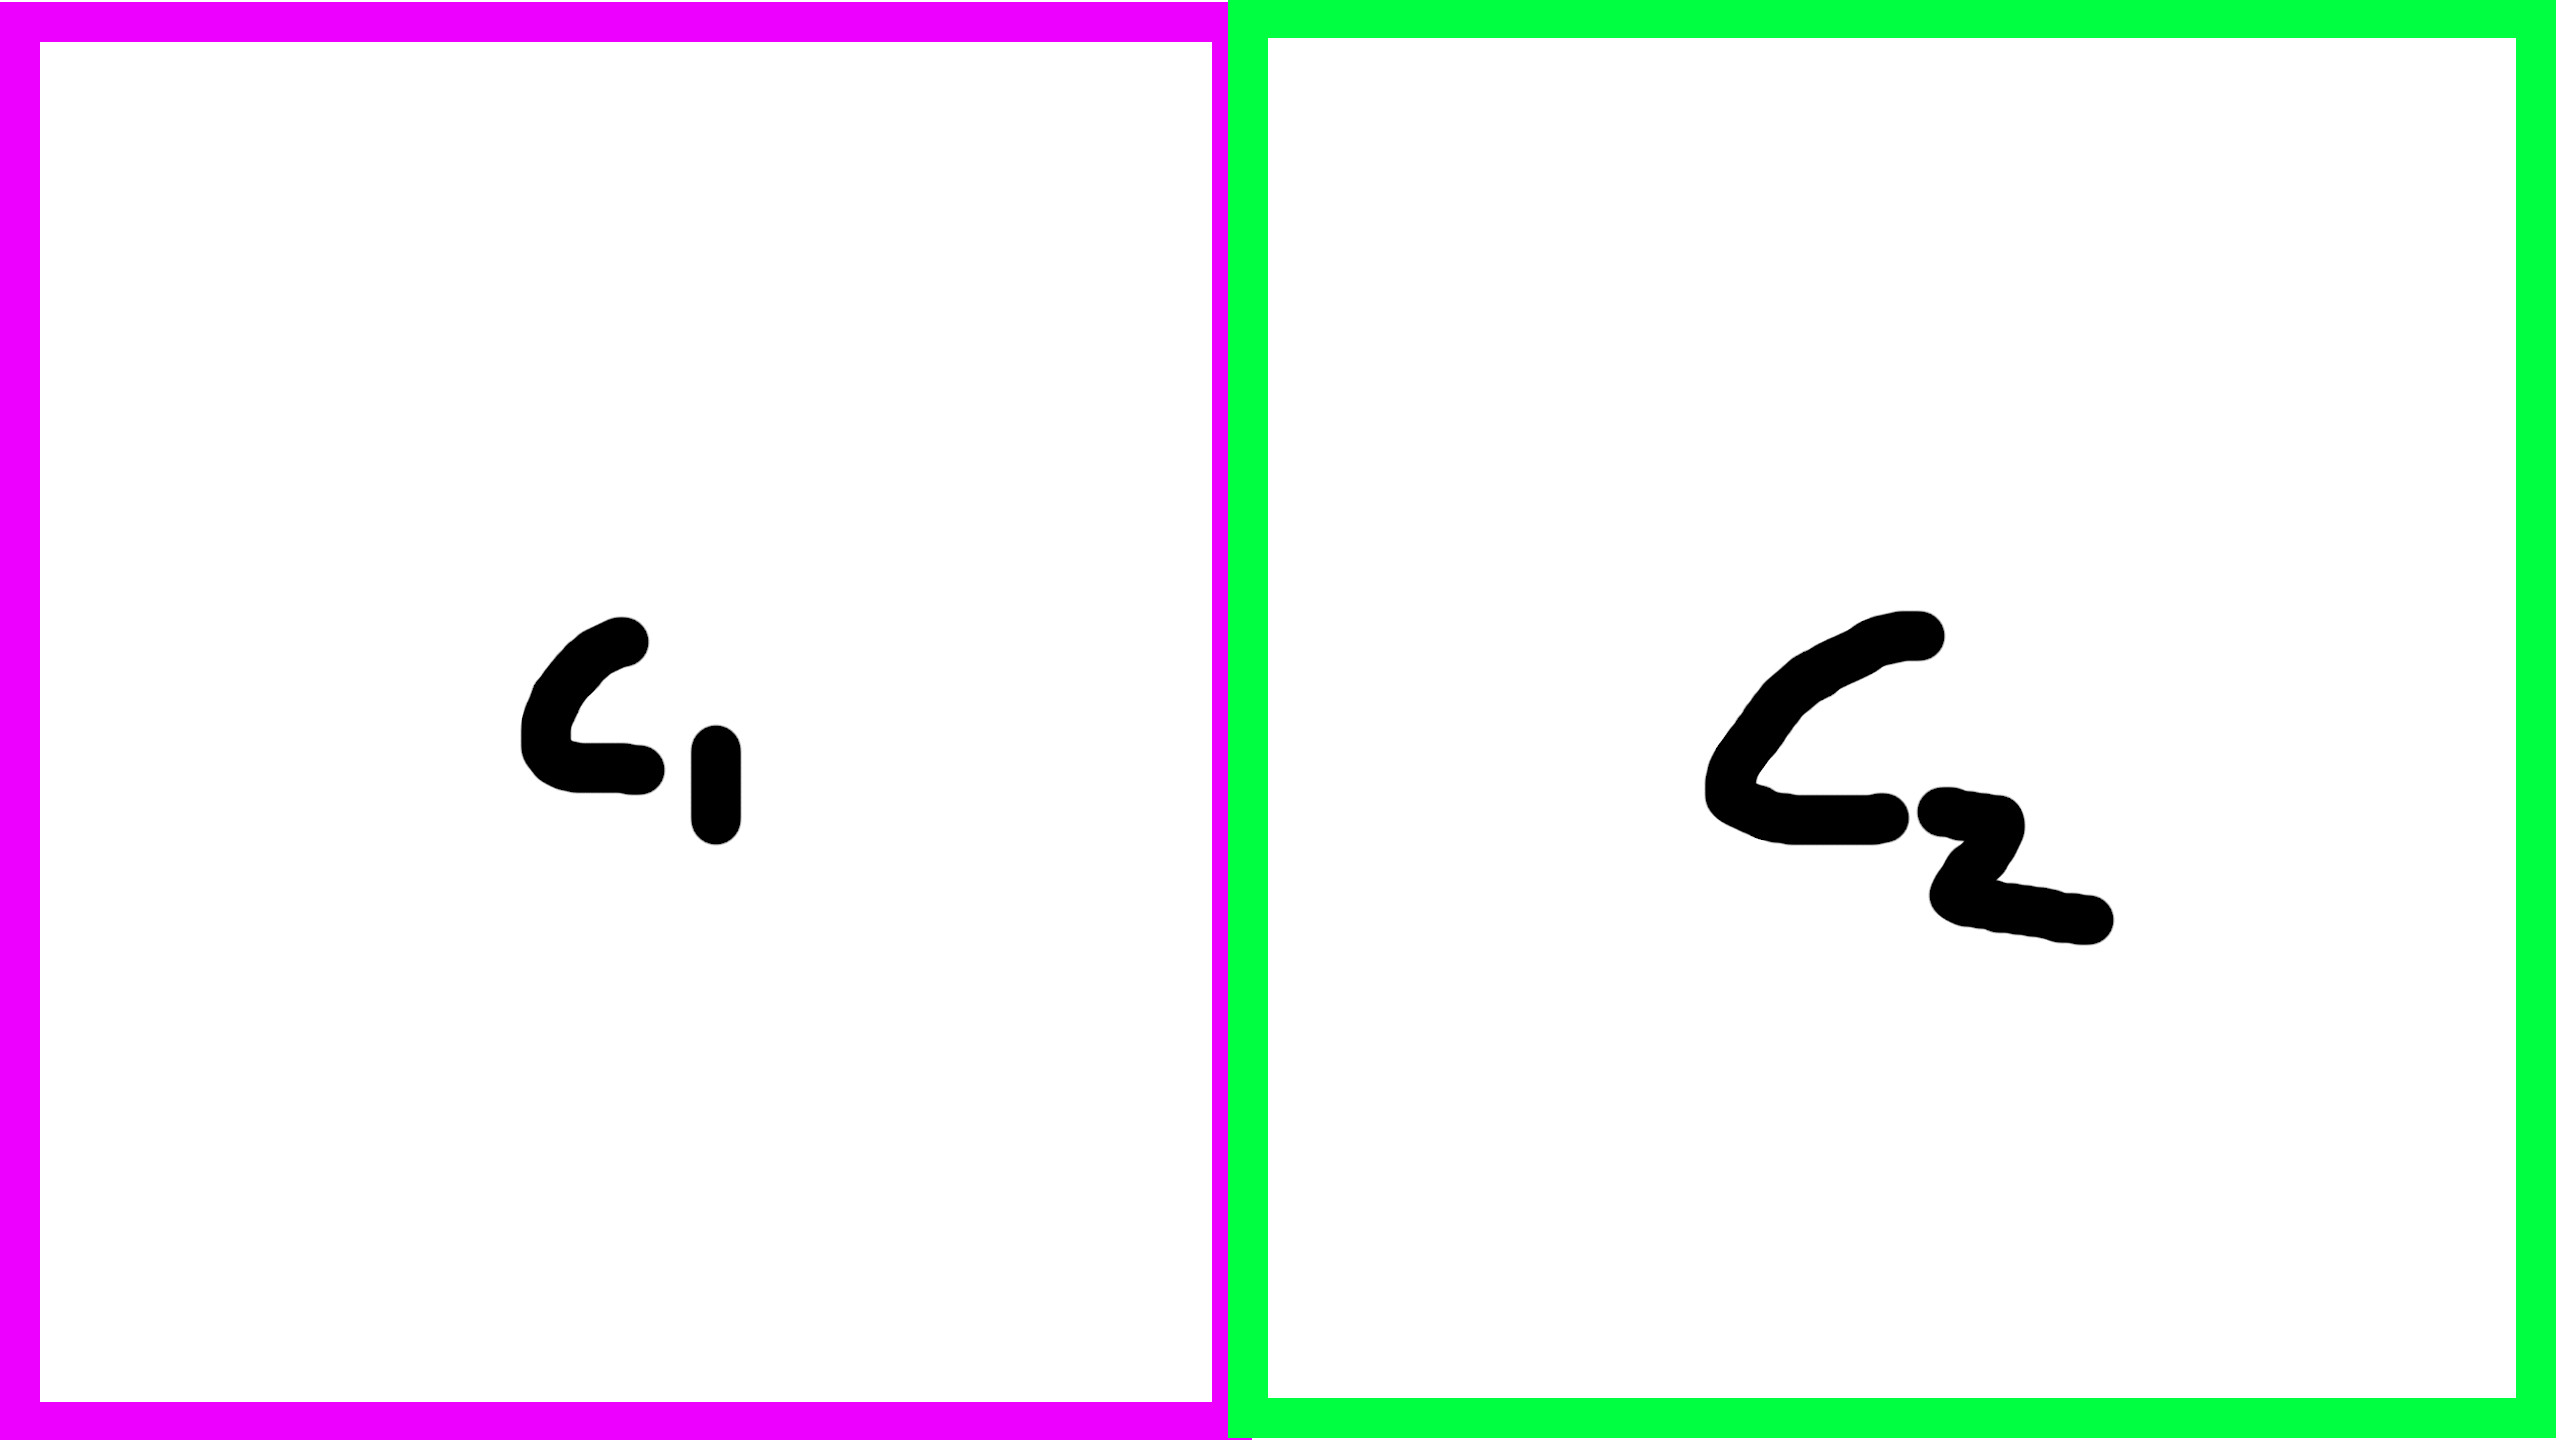
\includegraphics[height=0.2\textwidth]{figures/abstract-design.jpg}
    \label{fig: abstract model}
\end{figure}

Dentro de estas dos cajas, están los personajes que se han seleccionado y su color de traje, como se puede ver en la figura \ref{fig: strive chracter select}:

\begin{figure}[ht!]
    \centering
    \caption{Menú de selección de personaje de Guilty Gear Strive}
    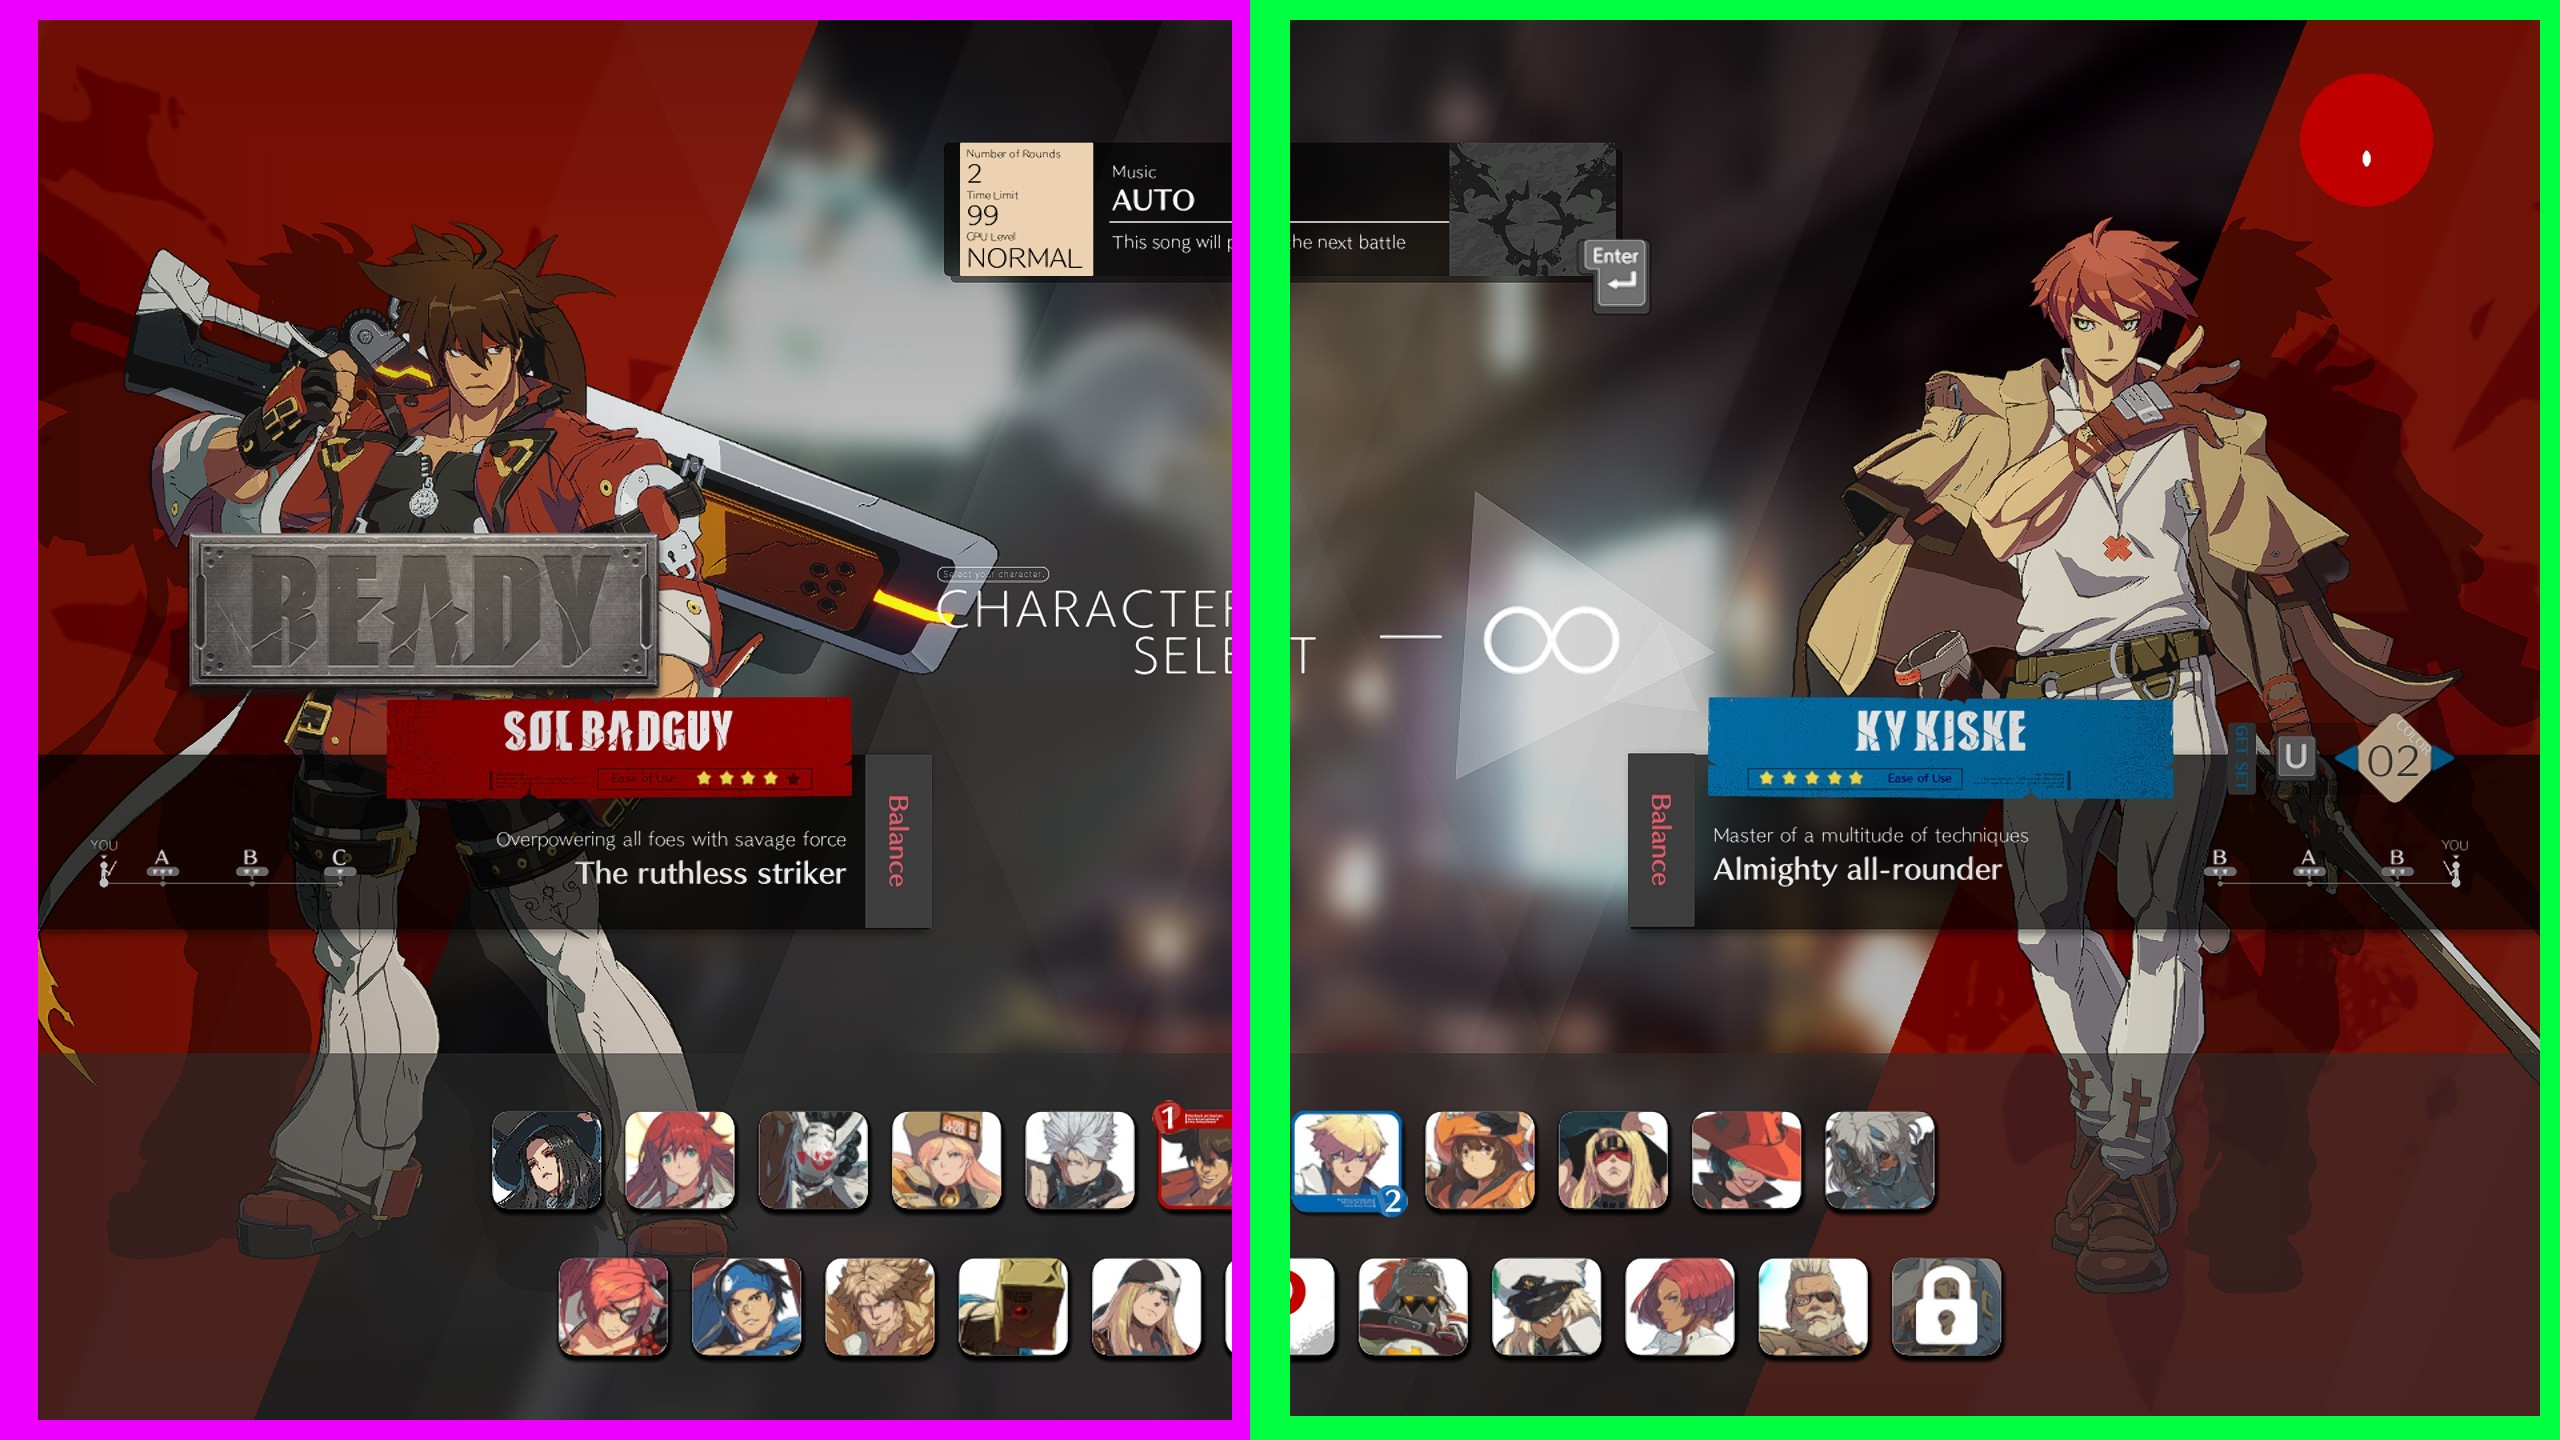
\includegraphics[height=0.5\textwidth]{figures/guilty.jpg}
    \label{fig: strive chracter select}
\end{figure}

Lo mismo ocurre en otros juegos como Melty Blood: Type Lumina \cite{noauthor_melty_nodate}, la figura \ref{fig: melty character select}:

\begin{figure}[ht!]
    \centering
    \caption{Menú de selección de personaje de Melty Blood}
    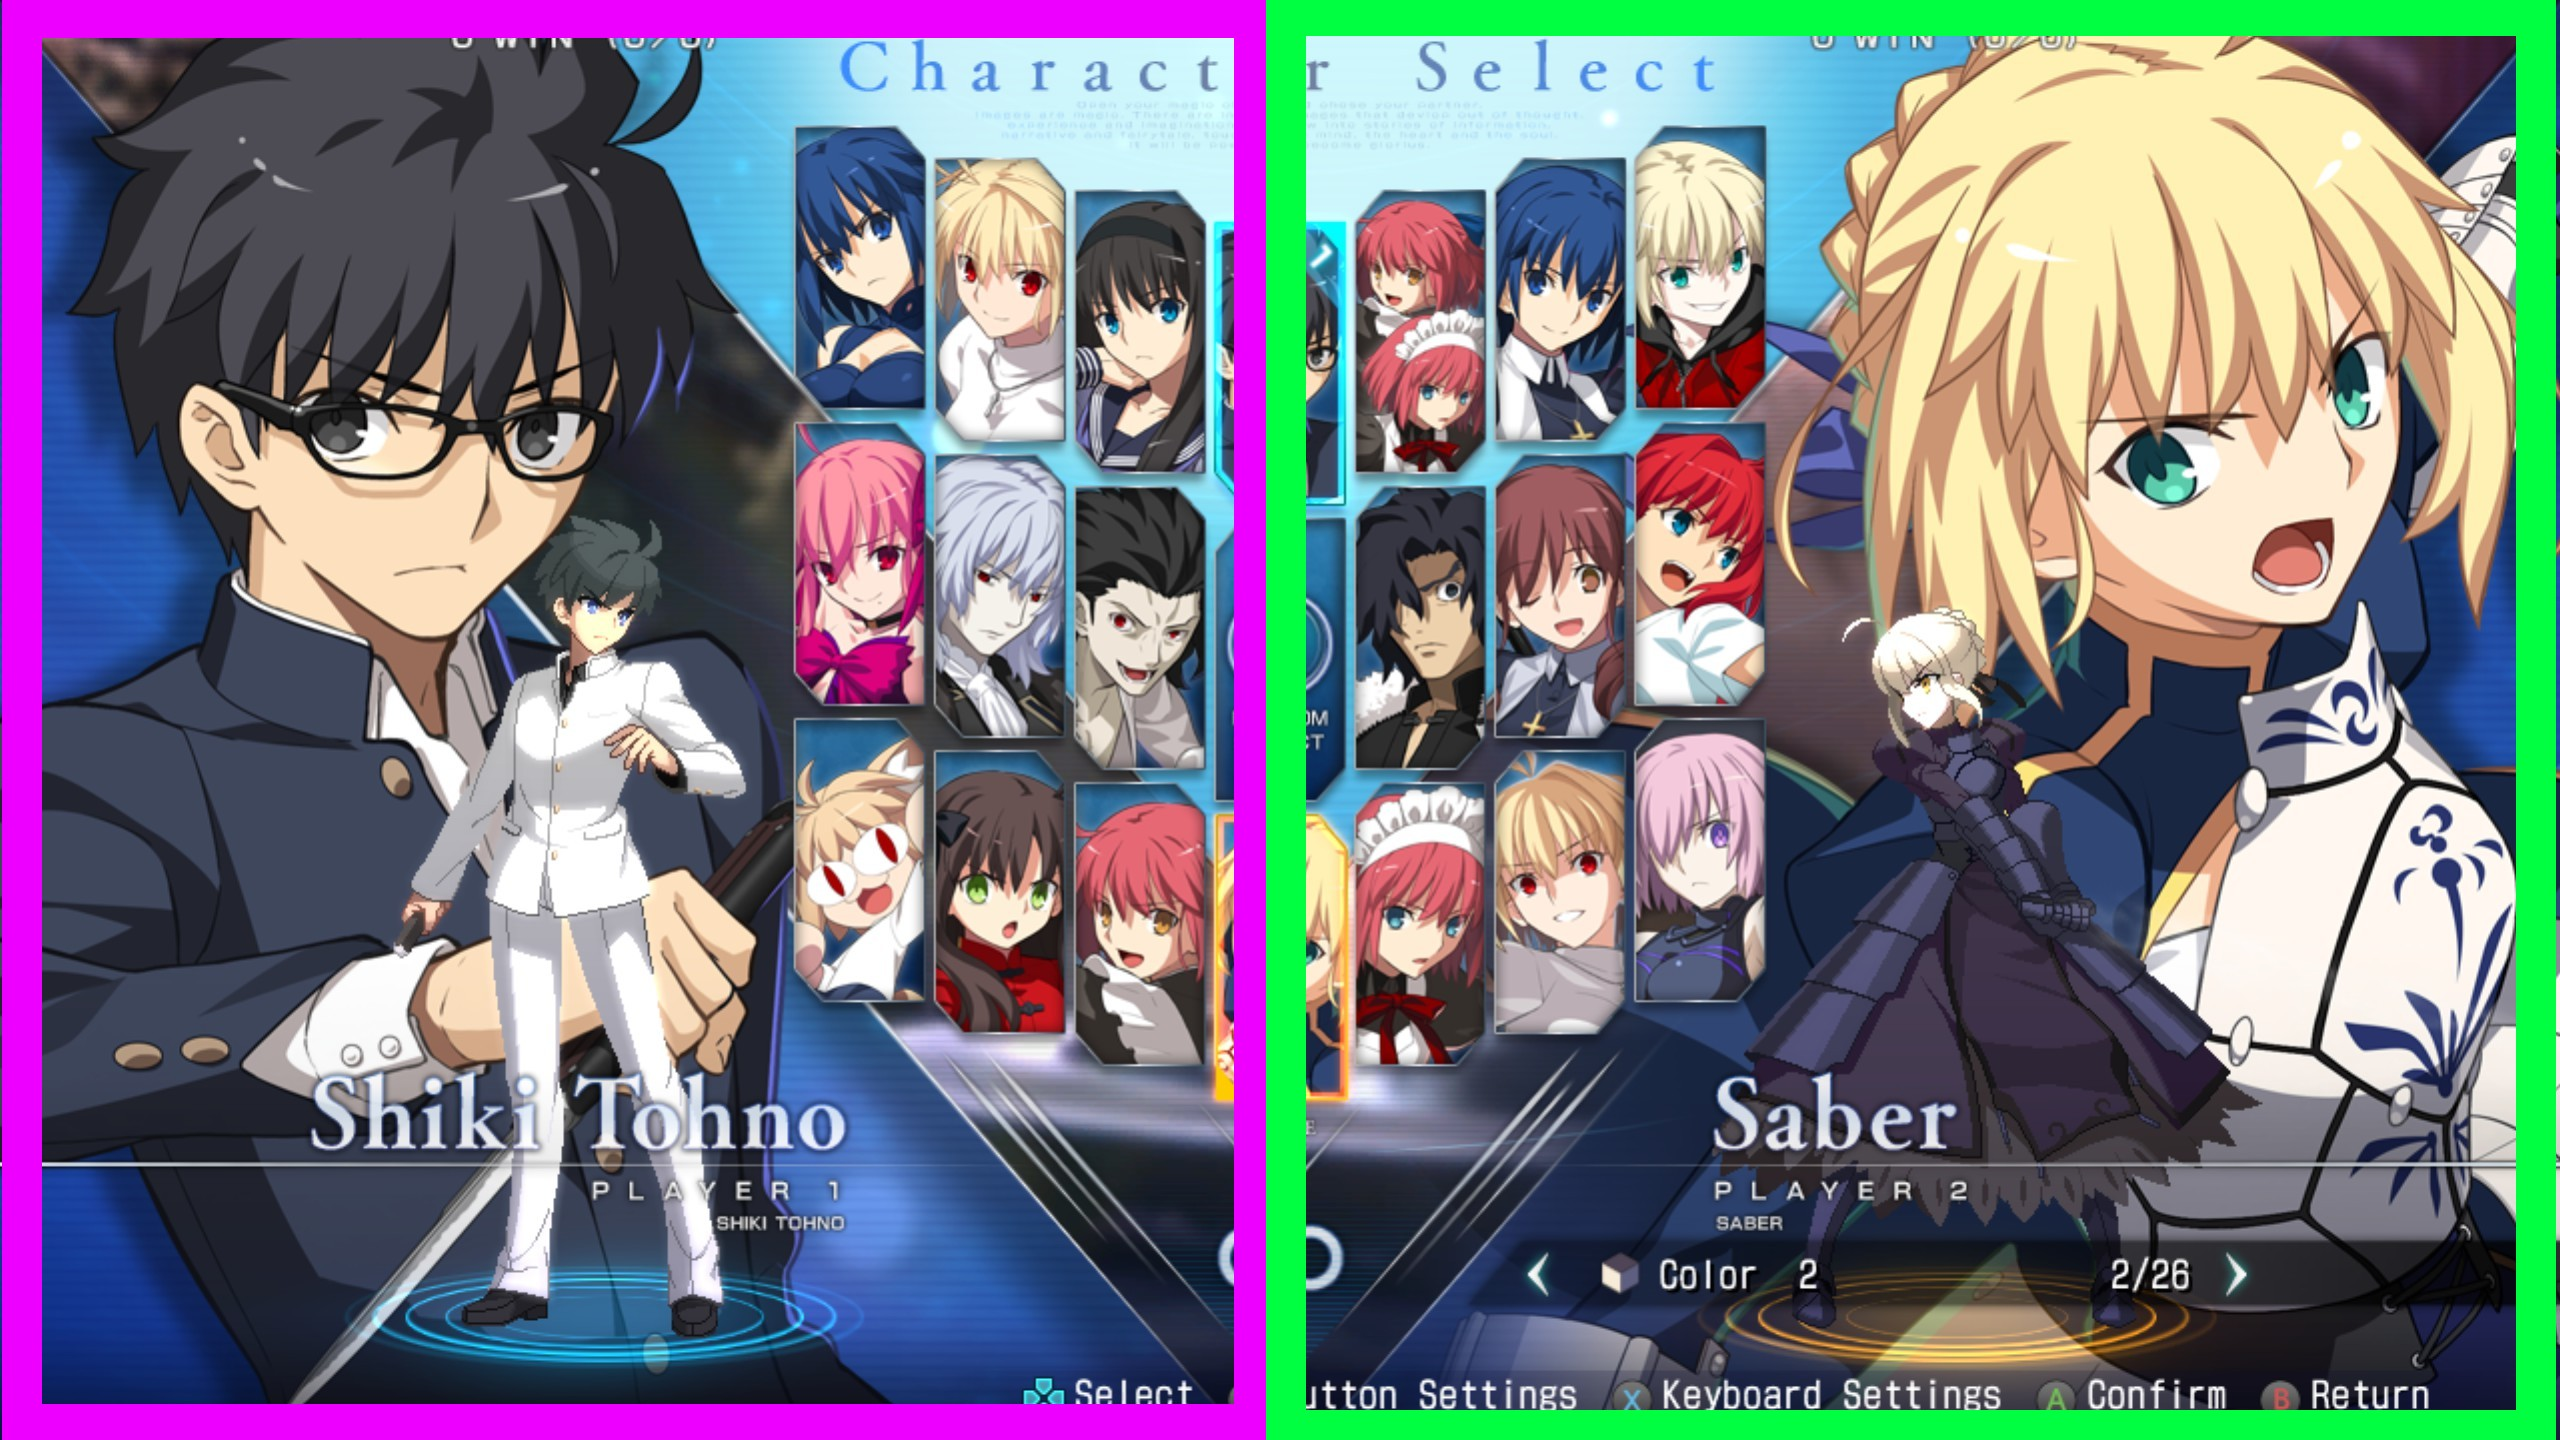
\includegraphics[height=0.5\textwidth]{figures/melty.jpg}
    \label{fig: melty character select}
\end{figure}

Como se ve en ambos ejemplos, los personajes seleccionados están colocados en esquinas opuestas, cada uno en su propia caja. El único elemento que se comparte entre los dos es la lista de personajes (caja azul)

\textbf{Características de la interfaz gráfica}: 

\begin{itemize}
    \item \textbf{Aspectos ergonómicos}
    \begin{itemize}
        \item El texto dentro de la aplicación tiene que ser legible
        \item Los menús desplegables tienen que ser lo suficientemente grande
        \item Se tiene que seguir los estándares de accesibilidad de HTML, tales como el uso de atributos \textit{alt} y el uso apropiado, lógico y consistente de etiquetas
        \item El botón de someter tiene que ser lo suficientemente claro en su propósito y suficientemente grande para que sea cómodo para todo tipo de usuario
    \end{itemize}
    \item \textbf{Colores}
    
    La paleta de colores es la siguiente:
    \begin{figure}[ht!]
        \centering
        \caption{Paleta de Colores}
        
\includegraphics[width=1.0\textwidth]{figures/pallete.png}
        \label{fig: pallete}
    \end{figure}

    Se utiliza el color del medio (\#3385D6 en hexadecimal) como color de fondo. Esto se debe a que al ser azul, distrae al usuario menos que un color como el rojo. Más aún, el color temático de \gls{gbfvs} es el azul claro. Esta relación ayuda a familiarizar el usuario con que juego esta trabajando esta aplicación. El color que se usa para los bordes es el color complementario de \#3385D6, el complemento de \#D69933 (marrón claro). Al marrón ser una mezcla del rojo y el verde, es bueno para detalles y para segmentar elementos de una manera visual.
    \item \textbf{Interactividad}
    \item \textbf{Validación de datos}
    
    Los fotogramas de cada personaje provienen de \textit{Dustloop} \cite{noauthor_granblue_2022-1}. Estos datos se extraen cada cierto periodo de tiempo de \textit{Dustloop} automáticamente. Se asume que debido a que \gls{gbfvs} ya no está recibiendo actualizaciones que \textit{Dustloop} no cambiará drásticamente la estructura de las páginas de donde se extrae la data. Por ende, se asume que la data fotográmica sera confiable por un buen tiempo.

    Debido a la naturaleza de los menús desplegables, no hay mucha validación necesaria en cuanto a las opciones que se le presentan al usuario. Sin embargo, hay un detalle importante que si se tiene que validar. La aplicación original de \textit{SkyboundDB} tiene la opción de comparar una movida con todas las movidas de otro personaje. Esto implica que no es posible comparar todas las movidas de un personaje con todas de otro por cuestiones de limpieza y por cuestiones prácticas debido a la cantidad de información que se tiene que presentar. A consecuencia de esto, se tiene que validar que el personaje que dio el primer golpe no tenga la opción de \textbf{Seleccionar todas las movidas} seleccionada y que el personaje que responde tampoco lo tenga a la vez. Solo el personaje que responde puede utilizar la opción de seleccionar todas sus movidas. Esta validación se tiene que hacer antes que se haga la comparación.
    % \item \textbf{Consistencia}
    \item \textbf{Carga de memoria}
    
    Idealmente, la carga de memoria debe ser baja por varias razones: Unas de las metas primordiales de este proyecto es que la aplicación sea rápida y eficiente. Unas de las métricas de eficiencia es la memoria primaria necesaria para mantener la página abierta. Otra métrica importante es la cantidad de banda ancha necesaria para acceder la página en linea. Unos de los casos de usos que tiene la aplicación es su uso en torneos, particularmente entre o antes de partidas. Esta circunstancia requiere que la pagina cargue rápidamente y sin tardarse mucho las comparaciones.  

    \item \textbf{Indicaciones visuales}
    
    Debido a las limitaciones de banda ancha, la página no puede tener una plantilla de estilo demasiada complicada. Sin embargo, elementos sencillos pueden mejorar la experiencia de usuario sin sacrificar mucho en términos de rapidez. Una imagen simple del personaje que se ha seleccionado, como se presenta en la figura \ref{fig: melty character select}, puede ayudar corroborar rápidamente si la selección del usuario fue la que quiso. Además, se puede estilizar la selección de movida para que se asemeje mas a la selección de traje como se puede apreciar con el dígito $2$ con las flechas en la parte derecha de las figuras \ref{fig: guilty character select} y \ref{fig: melty chracter select}. Estos detalles ayudan a conformarse al modelo mental que tiene el usuario de los juegos de pelea.
\end{itemize}